\section{Elementi di teoria dei numeri}

\subsection{Divisibilità e massimo comun divisore}

\begin{definition}[Divisibilità]
    \label{def:divisibilita}
    Si dice che $d$ divide $a$, e $a$ è multiplo di $d$ se,
    $
    \forall d \ne 0 \in \mathbb{Z}
    ,
    a \in \mathbb{Z}
    $
    \begin{equation*}
        d | a 
        \quad
        \text{se}
        \quad
        \exists k \in \mathbb{Z} : a = kd
    \end{equation*}
\end{definition}
\begin{definition}[Divisore]
    \label{def:divisore}
    Se $d$ divide $a$ e $d>0$ si dice che è divisore di $a$.
    Per esempio $-2$ divide $8$, mentre $2$ è divisore di $8$.
\end{definition}
Valgono le seguenti proposizioni riguardo alla divisibilità:
\begin{proposizione}
    $\forall d \in \mathbb{Z} - \left\{ 0 \right\}
    \Rightarrow
    d | 0$
\end{proposizione}
\begin{proposizione}
    $
    \left( d | a \right)
    \wedge
    \left( a \ne 0 \right)
    \Rightarrow
    |d| \leq |a|
    $
\end{proposizione}
\begin{corollario}
    \label{cor:divisore_limite}
    $
    \left( d | a \right)
    \wedge
    \left( a,d > 0 \right)
    \Rightarrow
    d \leq a
    $
\end{corollario}
\begin{proposizione}
    $
    \left( b | a \right)
    \wedge
    \left( a | b \right)
    \Rightarrow
    a = \pm b
    $ ovvero $
    |a| = |b|
    $
\end{proposizione}
\begin{definition}[Numero primo]
    \label{def:numeroprimo}
    $p > 1$ è primo se ha come divisori solo $1$ e $p$. Il numero $1$ non è considerato primo.
\end{definition}
\begin{theorem}[Divisione]
    \label{teo:divisione}
    Il teorema di divisione garantisce l'esistenza e l'unicità di quoziente e resto.
    \begin{equation*}
        \forall a \in \mathbb{Z}, \forall n \in \mathbb{Z}^+
        \quad
        \exists !
        \;
        q, r :
        a = qn + r
    \end{equation*}
    Dove $q$ è detto il quoziente della divisione intera
    \begin{equation*}
        q \in \mathbb{Z}
        \quad
        q = \left\lfloor 
            \frac{a}{n}
        \right\rfloor
        = a \divv n
    \end{equation*}
    E $r$ è detto resto della divisione intera
    \begin{equation*}
        r \in \mathbb{N}, 0 \leq r < n
        \quad
        r = a \bmod n
    \end{equation*}
\end{theorem}
\begin{corollario}
    Il teorema di divisione prova formalmente quello che si è già visto molto spesso per cui 
    \begin{equation*}
        -1 \bmod n = n-1
        \quad
        -1 = \left( -1 \right) n + \left( n-1 \right)
    \end{equation*}
\end{corollario}
\begin{definition} [Divisori comuni]
    \label{def:divisoricomuni}
    Dati $d > 0, a, b \in \mathbb{Z}$; $d$ è divisore comune di $a$ e $b$ se 
    $d|a$
    e
    $d|b$.
\end{definition}
\begin{proposizione}
    \label{prop:divisore_cli}
    Se $d$ è divisore comune di $a$ e $b$, è anche divisore di ogni loro combinazione lineare intera:
    \begin{equation*}
        \left( 
            d|a
        \right)
        \wedge
        \left( 
            d|b
        \right)
        \Rightarrow
        \forall x, y \in \mathbb{Z} :
        d | ax + by
    \end{equation*}
    \begin{proof}
        $d | a \leftrightarrow \exists k_a : a = k_a d$ 
        e
        $d | b \leftrightarrow \exists k_b : b = k_b d$ 
        allora si riscrive 
        $
        ax + by = k_a d x + k_b d y
        =
        \left( k_a x + k_b y \right) d
        $ e posto $
        k_d = 
        \left( k_a x + k_b y \right)
        $ vale $
        ax + by = k_d d
        $.
    \end{proof}
\end{proposizione}
\begin{definition} [Massimo comun divisore]
    \label{def:gcd}
    Siano $a, b \in \mathbb{Z} : |a| + |b| > 0$
    Il massimo comun divisore (\emph{greatest common divisor} o GCD) di $a$ e $b$ è
    \begin{equation*}
        gcd(a, b) = \max \left\{ 
            d > 0 :
            \left( 
                d|a
            \right)
            \wedge
            \left( 
                d|b
            \right)
        \right\}
    \end{equation*}
    L'ipotesi $|a| + |b| > 0$ garantisce che l'insieme sia limitato.
    Si pone per convenzione
    \begin{equation*}
        gcd(0,0) = 0
    \end{equation*}
\end{definition}
Valgono le seguenti proposizioni riguardo al GCD:
\begin{proposizione}
    \label{prop:gcd_bound}
    $ 
    |a| + |b| > 0
    \Rightarrow 
    1 \leq gcd(a,b)
    \leq \min \left\{ |a|, |b| \right\}
    $
\end{proposizione}
\begin{proposizione}
    \label{prop:gcd_zero}
    $ 
    \forall a \in \mathbb{Z}
    \Rightarrow 
    gcd(a,0) = |a|
    $ (anche per $a=0$ è coerente)
\end{proposizione}
\begin{proposizione}[Sign insensitivity]
    Vale
    \begin{equation*}
        gcd(a,b) =
        gcd(-a,b) =
        gcd(a,-b) =
        gcd(-a,-b) =
        gcd(|a|,|b|)
    \end{equation*}
    Questo permette di limitarsi allo studio dei naturali senza perdita di generalità.
\end{proposizione}

\subsection{Teorema di Bézout}

\begin{theorem} [Identità di Bézout]
    \label{teo:bezout}
    Sotto l'ipotesi $|a| + |b| > 0$, il GCD
    di $a$ e $b$
    è la minima combinazione lineare intera positiva 
    di $a$ e $b$.
    \begin{equation*}
        gcd(a,b) =
        \min \left\{ 
            d > 0 :
            \exists x, y \in \mathbb{Z} :
            d = ax + by
        \right\}
    \end{equation*}
    \begin{proof}
        Si mostra l'uguaglianza $
        gcd(a,b) = s
        $ dimostrando la minorazione e maggiorazione.
        \\
        ``$ gcd(a,b) \leq s $'':
        Per definizione di GCD vale $
        \left( 
            gcd(a,b) | a
        \right)
        \wedge
        \left( 
            gcd(a,b) | b
        \right)
        $
        e per la proprietà \ref{prop:divisore_cli} vale $
        gcd(a,b) 
        | ax + by
        ,
        \forall x, y \in \mathbb{Z}
        $.
        Se divide tutte le combinazioni lineari intere, deve dividere anche $s$:
        $
        gcd(a,b) | s
        $.
        Valgono le ipotesi della proposizione \ref{prop:gcd_bound} ($|a| + |b| > 0$), quindi $
        gcd(a,b) > 0
        $.
        Anche $s>0$ perché è il minimo di un insieme di numeri positivi.
        Entrambe le quantità sono positive e la prima divide la seconda, per cui dalla divisibilità discende $
        gcd(a,b) \leq s
        $ (corollario \ref{cor:divisore_limite}).
        \\
        ``$ gcd(a,b) \geq s $'':
        Prima di mostrare la minorazione, occorre dimostrare che
        \begin{equation*}
            \forall x, y \in \mathbb{Z}
            ,
            \;\;
            s | ax + by
        \end{equation*}
        Sia $
        s = a \bar{x} + b \bar{y}
        $ la combinazione minima e $
        c = ax + by
        $ una combinazione generica, si applica il teorema di divisione tra $c$ e $s$:
        \begin{equation*}
            \exists ! q, r :
            c = qs + r
            ,
            \quad
            0 \leq r < s
        \end{equation*}
        va mostrato che deve valere $r=0$, e quindi $s$ divide $c$.
        Si riscrive
        \begin{align*}
            r &= 
            c - qs
            \\
            &= 
            ax + by - q\left( 
                a \bar{x} + b \bar{y}
            \right)
            \\
            &= 
            a \left( 
                x - q \bar{x}
            \right)
            +
            b \left( 
                y - q \bar{y}
            \right)
            \\
            &=
            ax' + by'
        \end{align*}
        E si è mostrato che $r$ è combinazione lineare intera di $a$ e $b$.
        Ma $s$ era il minimo delle combinazioni lineari intere positive, quindi $r$ (che può assumere valori $
            0 \leq r < s
        $) non può essere positivo, perché avrebbe valore inferiore a $s$, e deve essere $r=0$.
        \\
        Avendo mostrato che $s$ divide ogni combinazione lineare intera, se ne possono scegliere due particolari:
        \begin{equation*}
            s | a \cdot 1 + b \cdot 0 = a
            \quad
            \text{e}
            \quad
            s | a \cdot 0 + b \cdot 1 = b
        \end{equation*}
        Ossia $s$ è divisore comune, minore o uguale al \emph{massimo} comun divisore: $
        gcd(a,b) \geq s 
        $.
    \end{proof}
\end{theorem}

\subsection{Teorema di Euclide}

Per il calcolo efficace del GCD si utilizza l'algoritmo di Euclide, considerato il primo esempio di algoritmo efficiente della storia.

\begin{theorem} [Euclide]
    \label{teo:euclide}
    Siano $a,b \geq 0$ (il GCD è invariante per segno, non si perde di generalità), allora
    \begin{align*}
        b=0
        &
        \Rightarrow
        gcd(a,b) =
        gcd(a,0) = a
        \\
        b>0
        &
        \Rightarrow
        gcd(a,b) =
        gcd(b,
            a \bmod b
        )
    \end{align*}
    \begin{proof}
        La prima implicazione è corrispondente alla proposizione \ref{prop:gcd_zero}.
        \\
        La seconda si prova in due parti:
        \\
        ``$ gcd(a,b) \leq gcd(b, a \bmod b) $'':
        Si applica il teorema di divisione ad $a$ e $b$:
        \begin{equation*}
            a = qb + r = qb + a \bmod b
            \quad
            \rightarrow
            \quad
            a \bmod b = a - qb
        \end{equation*}
        E si riscrive quindi
        \begin{align*}
            gcd(b, a \bmod b)
            &= 
            gcd(b, a - qb)
            % \intertext{a cui si applica il teorema di Bézout:
            % $ \exists x', y' \in \mathbb{Z} : $
            % }
            \\
            \text{per Bézout:
            $ \exists x', y' \in \mathbb{Z} : $
            }
            \quad
            &
            =
            b x' + 
            \left( 
                a - qb
            \right) y'
            \\
            &= 
            a y'
            +
            b
            \left( 
                x' - qy'
            \right)
        \end{align*}
        Per cui il $
        gcd(b, a \bmod b)
        $ è combinazione lineare intera positiva di $a$ e $b$ e sempre per Bézout, deve essere maggiore o uguale del $
        gcd(a, b)
        $, che è la minima combinazione lineare intera positiva:
        $ gcd(a,b) \leq gcd(b, a \bmod b) $.
        \\
        ``$ gcd(a,b) \geq gcd(b, a \bmod b) $'':
        Sia $
        d' = gcd(b, a \bmod b)
        $, allora valgono
        \begin{align*}
            d' | b 
            \Rightarrow
            \exists k' 
            &
            : b = k' d'
            \\
            d' | a \bmod b
            \Rightarrow
            \exists k'' 
            &
            : a \bmod b = k'' d'
        \end{align*}
        E si riscrive dal teorema di divisione
        \begin{align*}
            a
            &= 
            qb + a \bmod b
            \\
            &= 
            q k' d' 
            +
            k'' d'
            \\
            &= 
            \left( 
                q k' + k''
            \right) d'
        \end{align*}
        Quindi $
        \left( d' | a \right)
        $ e chiaramente $
        \left( d' | b \right)
        $, per cui $d'$ è divisore comune di $a$ e $b$, e deve essere minore del \emph{massimo} comun divisore.
    \end{proof}
\end{theorem}
Questo teorema mostra una chiara proprietà di sottostruttura, che riscrive la soluzione in funzione di istanze più piccole del problema.
\begin{algorithm}[H]
\caption{Algoritmo di Euclide}\label{alg:euclide}
\begin{algorithmic}[1]
    \Procedure{Euclid}{$a, b$}
        \If{$b = 0$}
            \State return $a$
        \EndIf
        \State return \Call{Euclid}{$b, a \bmod b$}
    \EndProcedure
\end{algorithmic}
\end{algorithm}
Se $a < b$ la prima iterazione scambia i valori ($
    a \bmod b = a
$), e alle successive iterazioni vale $b < a$ e quindi $a \bmod b < b$, essendo un minore stretto l'algortimo termina.
La correttezza dell'algoritmo è assicurata dal teorema precedente.

Per l'analisi della complessità, vanno introdotti i numeri di Fibonacci.
\begin{definition}
    [Numeri di Fibonacci]
    \label{def:numerifibonacci}
    I numeri di Fibonacci sono definiti come
    \begin{align*}
        F_1 &= 1
        \\
        F_2 &= 1
        \\
        F_{k+1}
        &=  
        F_{k} +
        F_{k-1}
        \quad
        \text{per}
        \quad
        k \geq 2
    \end{align*}
    Il cui valore è calcolabile in formula chiusa:
    \begin{align*}
        F_k &= 
        \frac{1}{
            \sqrt{5}
        }
        \left( 
            \frac{1 + 
                \sqrt{5}
            }{2}
        \right)^{k}
        -
        \frac{1}{
            \sqrt{5}
        }
        \left( 
            \frac{1 -
                \sqrt{5}
            }{2}
        \right)^{k}
        \\
        &
        \geq
        \frac{1}{
            2 \sqrt{5}
        }
        \left( 
            \frac{1 + 
                \sqrt{5}
            }{2}
        \right)^{k}
    \end{align*}
    I numeri di Fibonacci crescono come un esponenziale.
\end{definition}
Supponendo di conoscere il numero di chiamate $k$ eseguite dall'algoritmo di Euclide,
si trovano dei limiti inferiori per la grandezza dei parametri iniziali, dimostrando la velocità di convergenza dell'algoritmo.
% allora si dimostra che i parametri iniziali erano grandi rispetto al numero di chiamate.
\begin{lemma}
    \label{lem:euclide_iterazioni}
    Sia $k$ il numero di chiamate eseguite dall'algoritmo di Euclide, e siano $
    a > b > 0
    $, allora $
    a \geq F_{k+2}
    $ e $
    b \geq F_{k+1}
    $
    \begin{proof}
        La restrizione sugli input non è restrittiva:
        \begin{itemize}[noitemsep,parsep=0pt,partopsep=0pt,topsep=0pt]
            \item nel caso $a<b$ i valori vengono scambiati alla prima iterazione
            \item nel caso $a=b$ l'algortimo termina in due chiamate
            \item nel caso $b=0$ l'algortimo termina in una chiamata
        \end{itemize}
        I limiti si provano per induzione su $k$:
        \\
        Per $k=1$, vale 
        \begin{align*}
            a > b > 0
            \quad
            &
            \rightarrow
            b \geq 1 = F_2
            \\
            &
            \rightarrow
            a \geq 2 = F_3
        \end{align*}
        \\
        Sia vera l'ipotesi induttiva per $k-1$.
        \\
        Si analizza $\text{\textsc{Euclid}}(a,b)$ per $k>1$.
        $\text{\textsc{Euclid}}(b, a \bmod b)$ farà allora $k-1$ chiamate, e vale l'ipotesi induttiva:
        \begin{equation*}
            b \geq F_{(k-1)+2} = F_{k+1}
            \quad
            \text{e}
            \quad
            a \bmod b \geq F_{(k-1)+1} = F_{k}
        \end{equation*}
        Vale $a>b$ quindi per il teorema di divisione
        \begin{align*}
            a &= qb + a \bmod b
            \\
            \left( 
                q = \left\lfloor 
                    \frac{a}{b}
                \right\rfloor \geq 1
            \right)
            \quad 
            \quad 
            \quad 
            &
            \geq
            b + a \bmod b
            \\
            &
            \geq
            F_{k+1}
            +
            F_{k}
            \\
            &= 
            F_{k+2}
        \end{align*}
    \end{proof}
\end{lemma}
Avendo provato questo lemma, sia $
\bar{k}
$ il primo valore (minimo) per cui $
b < F_{
    \bar{k} + 1
}
$, allora $
b \geq F_{
    \bar{k}
}
$ e l'algoritmo non può fare più di $
\bar{k}
$ chiamate.
\begin{align*}
    b
    &
    \geq F_{
        \bar{k}
    }
    \geq
    \frac{1}{
        2 \sqrt{5}
    }
    \left( 
        \frac{1 + \sqrt{5} }{2}
    \right)^{k}
    \\
    \log_{ \frac{1 + \sqrt{5} }{2} }
    b
    &
    \geq
    \bar{k}
    +
    \log_{ \frac{1 + \sqrt{5} }{2} }
    \frac{1}{ 2 \sqrt{5} }
    \\
    \bar{k}
    &
    \leq
    \log_{ \frac{1 + \sqrt{5} }{2} }
    b
    -
    \log_{ \frac{1 + \sqrt{5} }{2} }
    \frac{1}{ 2 \sqrt{5} }
\end{align*}
Quindi a meno di costanti vale
\begin{equation*}
    T_{euclid} \left( a, b \right)
    =
    \bar{k}
    =
    O \left( \log b \right)
    =
    O \left( |
        \langle
            a, b
        \rangle 
    | \right)
\end{equation*}
Note:
\\
Il valore di $a$ è irrilevante, alla prima iterazione viene abbattuto da $b$.
\\
L'algoritmo è veloce ma non troppo, infatti ad ogni iterazione va effettuata un'operazione di modulo, che è quadratica nella taglia dei numeri considerati.
La complessità risulta
$
O
% \left( \left( \log b \right)^3 \right)
( ( \log b )^3 )
$, e considerando che si utilizzano in genere numeri a migliaia di bit, non è trascurabile nelle applicazioni pratiche.

\subsubsection{Calcolo del valore del GCD}

Il massimo comun divisore è una precisa combinazione lineare dei due valori di ingresso.
\begin{equation*}
    gcd(a, b) = a \bar{x} + b \bar{y}
\end{equation*}
Si può modificare l'algoritmo di Euclide in modo da ricavare i valori di $
\bar{x}
$ e $
\bar{y}
$.
Per il caso base $b=0$:
\begin{equation*}
    gcd(a, 0) = a = a \cdot 1 + b \cdot 0
\end{equation*}
L'algoritmo modificato ritorna una \texttt{struct} formata da $
\left\{ a, \left( 1, 0 \right) \right\}
$.
\\
Per il caso generico:
dal teorema della divisione 
\begin{equation*}
    a = 
    \left\lfloor \frac{a}{b} \right\rfloor
    b
    +
    a \bmod b
    \quad
    \rightarrow
    \quad
    a \bmod b
    =
    a -
    \left\lfloor \frac{a}{b} \right\rfloor
    b
\end{equation*}
E quindi sostituendo
\begin{align*}
    gcd(a,b)
    &= 
    gcd(b,
        a \bmod b
    )
    \\
    &= 
    b x' + \left( 
        a \bmod b
    \right) y'
    \\
    &= 
    b x' + \left( 
        a -
        \left\lfloor \frac{a}{b} \right\rfloor
        b
    \right) y'
    \\
    &= 
    a y' +
    \left( 
        x' +
        \left\lfloor \frac{a}{b} \right\rfloor
        y'
    \right) b
    \\
    &= a \bar{x} + b \bar{y}
\end{align*}
Si estende facilmente l'algoritmo di Euclide in modo da costruire i valori man mano:
\begin{algorithm}[H]
\caption{Algoritmo di Euclide esteso}\label{alg:euclide_extended}
\begin{algorithmic}[1]
    \Procedure{EE}{$a, b$}
        \If{$b = 0$}
            \State return $ \left\{ a, \left( 1, 0 \right) \right\} $
        \EndIf
        \State $ \left\{ d, \left( x', y' \right) \right\} 
        \gets
        $ \Call{EE}{$b, a \bmod b$}
        \State return $ \left\{ d, \left( y', x' - a \divv b \cdot y' \right) \right\} $
    \EndProcedure
\end{algorithmic}
\end{algorithm}

\section{Aritmetica modulare}

% Valgono le seguenti proprietà del modulo:
\subsection{Proprietà del modulo}

\begin{proposizione}
    \label{prop:distri_mod_add}
    Proprietà distributiva rispetto all'addizione:
    \begin{equation*}
        \left( a+b \right)
        \bmod n 
        =
        \left( 
            \left( 
                a \bmod n
            \right)
            +
            \left( 
                b \bmod n 
            \right)
        \right)
        \bmod n 
    \end{equation*}
\end{proposizione}

\begin{proposizione}
    Proprietà distributiva rispetto alla moltiplicazione:
    \begin{equation*}
        \left( a \cdot b \right)
        \bmod n 
        =
        \left( 
            \left( 
                a \bmod n
            \right)
            \cdot
            \left( 
                b \bmod n 
            \right)
        \right)
        \bmod n 
    \end{equation*}
\end{proposizione}

\begin{proposizione}
    \label{prop:mod_differenza}
    \begin{equation*}
        a \bmod n = b \bmod n 
        \quad
        \Leftrightarrow
        \quad
        ( a - b ) \bmod n = 0
        \quad
        \Leftrightarrow
        \quad
        \exists k \in \zz{}
        :
        a - b = kn
    \end{equation*}
\end{proposizione}

\begin{proposizione}
    \label{prop:mod_elimina_interno}
    Se $m | n$ e $m, n > 0$:
    \begin{equation*}
        \exists x \in \zz{}
        :
        \left( 
            x \bmod n 
        \right)
        \bmod m
        =
        x \bmod m
    \end{equation*}
\end{proposizione}

Si dimostra la proposizione \ref{prop:distri_mod_add}, le altre sono lasciate per ESERCIZIO.
\begin{proof}
    Applicando il teorema di divisione
    \begin{align*}
        a + b
        = 
        q_1 \, n + r_1
        &
        &
        r_1  
        &
        =
        ( a + b )
        \bmod n 
        \\
        a
        = 
        q_a \, n + r_a
        &
        &
        r_a  
        &
        =
        a
        \bmod n 
        \\
        b
        = 
        q_b \, n + r_b
        &
        &
        r_b  
        &
        =
        b
        \bmod n 
        \\
        r_a + r_b
        = 
        q_{ab} \, n + r_2
        &
        &
        r_2  
        &
        =
        ( r_a + r_b )
        \bmod n 
        \\
        &
        &
        &
        =
        ( ( a \bmod n ) + ( b \bmod n ) ) \bmod n 
    \end{align*}
    Quindi per provare la proprietà deve valere $
    r_1 = r_2
    $
    \begin{align*}
        a + b
        &
        =
        \left( 
            q_a n + r_a
        \right)
        +
        \left( 
            q_b n + r_b
        \right)
        \\
        &
        =
        \left( 
            q_a + q_b + q_{ab}
        \right) n +
        r_2
    \end{align*}
    Il teorema di divisione assicura l'esistenza e l'\emph{unicità} di $q$ e $r$, per cui
    \begin{equation*}
        q_a + q_b + q_{ab} = q_1
        \quad
        r_1 = r_2
    \end{equation*}
\end{proof}

\subsection{Strutture quozienti}

\begin{definition}
    [Congruo]
    \label{def:congruo}
    Se $a, b \in \zz{}$, si dice che $a$ è congruo a
    % $b \bmod n $ se
    $b$ modulo $ n $ se
    \begin{equation*}
        a \equiv b \bmod n 
        \quad
        \Leftrightarrow
        \quad
        a \equiv_n b
        \quad
        \Leftrightarrow
        \quad
        a \bmod n + b \bmod n 
    \end{equation*}
\end{definition}
La relazione $
    \equiv_n
$ è riflessiva ($
    a \equiv_n a
$), è simmetrica ($
    a \equiv_n b
    \Leftrightarrow
    b \equiv_n a
$) ed è transitiva ($
    ( a \equiv_n b )
    \wedge
    ( b \equiv_n c )
    \Rightarrow
    ( a \equiv_n c )
$), quindi è una relazione d'equivalenza, che induce una partizione di $
    \zz{}
$ in classi di equivalenza.
\begin{definition}
    [Classe di equivalenza]
    La classe di equivalenza $
    \cln{a} 
    $ è formata dagli interi congrui ad $a$.
    \begin{equation*}
        \cln{a}
        =
        \left\{ 
            x \in \zz{}
            :
            x \equiv_n a
        \right\}
    \end{equation*}
\end{definition}
Fissata $
\cln{a} 
$, per gli elementi della classe vale
\begin{align*}
    x \equiv_n a
    &
    \Leftrightarrow
    x \bmod n + a \bmod n 
    \\
    \text{(prop \ref{prop:mod_differenza})}
    \quad
    &
    \Leftrightarrow
    ( x - a ) \bmod n = 0
    \intertext{ Per cui il resto della divisione intera tra $x-a$ e $n$ è nullo, e vale }
    x - a = q n
    \quad
    &
    \Rightarrow
    \quad
    x = a + q n
\end{align*}
La classe si riscrive come la progressione aritmetica
\begin{equation*}
    \cln{a}
    =
    \left\{ 
        a + qn : q \in \zz{}
    \right\}
\end{equation*}
Ed è invariante per il rappresentante:
% se $
$ \forall x \in \zz{} : 
    x \equiv_n a
$ vale
\begin{equation*}
    \cln{a}
    =
    \left\{ 
        x + qn : q \in \zz{}
    \right\}
\end{equation*}

\begin{definition}
    [Insieme delle classi di equivalenza]
    L'insieme delle classi di equivalenza è l'insieme degli insiemi
    \label{def:insieme_classi_equiv}
    \begin{equation*}
        \zz{n} =
        \left\{ 
            \cln{i}
            : 0 \leq i \leq n-1
        \right\}
    \end{equation*}
\end{definition}
Dato $n$, ci sono chiaramente $n$ classi di equivalenza.
I valori $0, 1, \dots, n-1$ sono detti rappresentanti principali delle classi.
I rappresentanti principali sono elementi di $\zz{}$.  
\\
Per convenzione, si indicano le classi con i loro rappresentanti principali 
\begin{equation*}
    a \in \zz{n}
    \quad
    \leftrightarrow
    \quad
    \cln{a} \in \zz{n}
\end{equation*}

Vengono definite due operazioni tra classi di equivalenza:
\begin{align*}
    % \oplus : 
    % \zz{n}
    % \times
    % \zz{n}
    % \to
    % \zz{n}
    % \ni
    \quad
    \cln{a} 
    \oplus
    \cln{b} 
    &
    =
    \cln{a + b}
    \\
    % \odot : 
    % \zz{n}
    % \times
    % \zz{n}
    % \to
    % \zz{n}
    % &
    \quad
    \cln{a} 
    \odot
    \cln{b} 
    &
    =
    \cln{a \cdot b}
\end{align*}
Per esempio
$
7 \in \cleq{5}{2}
$ ($
    7 \bmod 5 = 2
$) e
$
9 \in \cleq{5}{4}
$ ($
    9 \bmod 5 = 4
$).
La somma tra classi risulta
$
\cleq{5}{2}
\oplus
\cleq{5}{4}
=
\cleq{5}{1}
$
e infatti
$
7 + 9 = 16 \in \cleq{5}{1}
$ ($
    16 \bmod 5 = 1
$).
\\
Quando si usa la notazione compatta, va ricordato che le operazioni sono tra classi, mentre i rappresentanti sono interi:
\begin{equation*}
    \zz{n} \times \zz{n} \ni
    a \oplus b = ( a + b ) \bmod n 
\end{equation*}
Va quindi tenuto conto del fatto che gli insiemi $\cln{a} $ sono sempre insiemi infiniti,
e le operazioni che si compiono devono quindi essere coerenti con l'invarianza del rappresentante.
\\
Scrivendo il rappresentante generico della somma si mostra la sua invarianza rispetto al rappresentante.
\begin{align*}
    \cln{a} 
    \oplus
    \cln{b} 
    &
    =
    \cln{a + q_1 n} 
    \oplus
    \cln{b + q_2 n} 
    \\
    &
    =
    \cln{ ( a + b ) + ( q_1 + q_2 ) n} 
    \\
    &
    =
    \cln{a + b}
\end{align*}

\subsection{Proprietà di gruppo di $\zz{n}$}

\subsubsection{Gruppo additivo}

L'insieme
delle classi di equivalenza è un gruppo additivo (abeliano)
rispetto alla somma
$
\left( 
    \zz{n}, \oplus
\right)
$.

\begin{itemize}
    \item esiste l'elemento neutro $
        \cln{0}
        $, infatti
        $
        \forall \cln{a} \in \zz{n} 
        $
        vale
        $
        \cln{a} \oplus \cln{0} = \cln{a} 
        $
    \item l'associatività si eredita dalla somma tra interi
    \item per la chiusura, l'operazione $\oplus$ ha sempre come risultato una classe in $\zz{n} $
    \item esiste l'inverso additivo (opposto):
        l'inverso di $
        \cln{a}
        $
        è
        $
        \cln{-a} 
        $,
        il cui rappresentante principale è $
        ( -a ) \bmod n = ( n - a ) \bmod n 
        $ e vale $
        \cln{-a} 
        \oplus 
        \cln{a} 
        =
        \cln{0} 
        $
\end{itemize}

\subsubsection{Gruppo moltiplicativo}

L'elemento neutro per $\odot $ è chiaramente $
\cln{1} 
$.

Di sicuro
$
\left( 
    \zz{n}, \odot
\right)
$
non è un gruppo, perché $
\cln{0} 
$ non ha inverso.

Anche
$
\left( 
    \zz{n} - \left\{ 
        \cln{0} 
    \right\}
    , \odot
\right)
$ non è un gruppo moltiplicativo, perché di nuovo alcuni elementi non hanno l'inverso:
si consideri $
\zz{4}
$, qual è l'inverso di $
\cleq{4}{2}
$? Lo si cerca per enumerazione:
\begin{align*}
    \cleq{4}{2}
    \odot
    \cleq{4}{0}
    &= 
    \cleq{4}{0}
    &
    \cleq{4}{2}
    \odot
    \cleq{4}{1}
    &= 
    \cleq{4}{2}
    \\
    \cleq{4}{2}
    \odot
    \cleq{4}{2}
    &= 
    \cleq{4}{0}
    &
    \cleq{4}{2}
    \odot
    \cleq{4}{3}
    &= 
    \cleq{4}{2}
\end{align*}
Nessuno di questi risulta $
    \cleq{4}{1}
$ quindi $
    \cleq{4}{2}
$ non ha inverso in $
\zz{4}
$.

Si considerano allora solo le classi i cui rappresentanti principali sono primi con $n$.
\begin{equation*}
    \zs{n}
    =
    \left\{ 
        \cln{a} 
        \in \zz{n} 
        :
        gcd(a, n) = 1
    \right\}
\end{equation*}
Per prima cosa va verificato se $
\zs{n} 
$ sia ben definito, ovvero se sia invariante rispetto al rappresentante principale.
Lo si dimostra usando Bézout:
\begin{align*}
    1 = 
    gcd(a, n)
    &
    = 
    ax + ny
    \\
    &
    = 
    ax + ny + qnx - qnx
    \\
    &
    = 
    \left( a + qn \right) x
    +
    n \left( y - qx \right)
    % \\
    % &
    % =
    % gcd(a + qn, n)
\end{align*}
Quindi si è scritto $1$ come combinazione lineare tra $
a + qn
$ e $n$. Di nuovo per Bézout, la minima combinazione lineare è il GCD, e non può essercene una minore, per cui $
    gcd(a + qn, n) = 1
$. $
a + qn
$ è il generico rappresentante, e si conclude.

Le proprietà di un gruppo sono verificate:
\begin{itemize}
    \item esiste l'elemento neutro $
        \cln{1}
        $
    \item l'associatività si eredita dal prodotto tra interi
    \item per la chiusura deve valere
        \begin{align*}
            \left( 
                gcd(a, n) = 1
            \right)
            &
            \wedge
            \left( 
                gcd(b, n) = 1
            \right)
            \quad
            \Rightarrow
            \quad
            gcd(ab, n) = 1
            \shortintertext{che si dimostra con Bézout:}
            1 &= a x_a + n y_a
            \\
            1 &= b x_b + n y_b
            \shortintertext{e moltiplicando membro a membro}
            1 \cdot 1 &= a b x_a x_b
            + n (\ldots)
            + n (\ldots)
            + n^2 (\ldots)
            \shortintertext{raccogliendo $n$ si ottiene una combinazione lineare di $ab$ e $n$, e si riapplica Bézout}
            &= a b \bar{x} + n \bar{y}
        \end{align*}
    \item riguardo all'esistenza e unicità dell'inverso moltiplicativo $
        \left( 
            \cln{a} 
        \right)^{-1}
        $ di $
        \cln{a} 
        $, da Bézout si ricava
        \begin{align*}
            1 = ax + ny
            \quad
            \rightarrow
            \quad
            ax
            &
            = 1 - ny
            \shortintertext{prendendo il modulo}
            \left( 
                ax
            \right)
            \bmod n 
            &
            =
            \left( 
                1 - ny
            \right)
            \bmod n 
            \shortintertext{applicando la distributiva}
            \left( 
                \left( 
                    a \bmod n
                \right)
                \left( 
                    x \bmod n 
                \right)
            \right)
            \bmod n 
            &= 
            \left( 
                \left( 
                    1 \bmod n
                \right)
                +
                \left( 
                    \left( -ny \right)
                    \bmod n 
                \right)
            \right)
            \bmod n 
            \shortintertext{
                al secondo membro valgono
                $
                1 \bmod n = 1 
                $
                e 
                $
                \left( -ny \right) \bmod n = 0 
                $
            }
            \left( 
                \left( 
                    a \bmod n
                \right)
                \left( 
                    x \bmod n 
                \right)
            \right)
            \bmod n 
            &= 1
            % \shortintertext{per cui la classe il cui rappresentante principale è $x \bmod n $ è l'inverso moltiplicativo della classe di $a$, il cui rappresentante principale è $a \bmod n $ }
        \end{align*}
        per cui la classe il cui rappresentante principale è $x \bmod n $
        è l'inverso moltiplicativo della classe di $a$, il cui rappresentante principale è $a \bmod n $,
        ovvero $
        x \bmod n
        $ è il rappresentante principale della classe $
        \left( \cln{a} \right)^{-1}
        $.
        \\
        Va ora verificato che $
        \cln{x} \in \zs{n} 
        $: sempre per Bézout vale
        \begin{align*}
            gcd(a, n) = 1
            \rightarrow
            1 &=  ax + ny
            \\
            1 &=  xa + ny
            \rightarrow
            gcd(x, n) = 1
        \end{align*}
        La prova dell'unicità è lasciata per ESERCIZIO, si mostra che se
        $ \cln{a} \odot \cln{x} = \cln{1} $
        e
        $ \cln{a} \odot \cln{y} = \cln{1} $
        allora 
        $\cln{x} = \cln{y}$.
        Una proprietà utile, che pure va dimostrata, è la seguente $
        \left( ab | n \right)
        \wedge
        \left( gcd(a, n) = 1 \right)
        \Rightarrow
        \left( b | n \right)
        $ (intuitivamente, se $ab$ divide $n$ ma $a$ e $n$ non hanno divisori in comune, deve essere $b$ che moltiplica $a$ per ottenere $n$).
\end{itemize}
Il coefficiente della combinazione lineare si ottiene con l'algoritmo esteso di Euclide:
\begin{algorithm}[H]
\caption{Inverso moltiplicativo}\label{alg:inverse}
\begin{algorithmic}[1]
    \Procedure{Inverse}{$a, n$}
        \State $\left\{ d, \left( x, y \right) \right\} \gets $ \Call{EE}{$a, n$}
        \State return $x \bmod n$
    \EndProcedure
\end{algorithmic}
\end{algorithm}

Per esempio,
l'algoritmo per $
\cleq{15}{4}
\in
\zs{15} 
$
esegue le seguenti chiamate,
ricordando che l'algoritmo esteso di Euclide 
EE($a, b$)
ritorna
\begin{align*}
    &
    \left\{ d, \left( y', x' - a \divv b \cdot y' \right) \right\}
    \quad
    \text{se}
    \quad
    \left\{ d, \left( x', y' \right) \right\} \gets \text{EE} (b, a \bmod b)
    \\
    &
    \text{EE} ( 15, 4)
    \\
    &
    \quad
    \text{EE} (4,  15 \bmod 4 = 3)
    \\
    &
    \quad
    \quad
    \text{EE} (3,  4 \bmod 3 = 1)
    \\
    &
    \quad
    \quad
    \quad
    \text{EE} (1,  3 \bmod 1 = 0)
    \\
    &
    \quad
    \quad
    \quad
    \quad
    \text{return} \left\{ 1, \left( 
            1, 0
    \right) \right\}
    \quad
    \text{(caso base)}
    \\
    &
    \quad
    \quad
    \quad
    \text{return}
    \left\{ 1, \left( 
            0, 1 - \left\lfloor 3/1 \right\rfloor \cdot 0
    \right) \right\}
    =
    \left\{ 1, \left( 
            0, 1
    \right) \right\}
    \\
    &
    \quad
    \quad
    \text{return}
    \left\{ 1, \left( 
            1, 0 - \left\lfloor 4/3 \right\rfloor \cdot 1
    \right) \right\}
    =
    \left\{ 1, \left( 
            1, -1
    \right) \right\}
    \\
    &
    \quad
    \text{return}
    \left\{ 1, \left( 
            -1, 1 - \left\lfloor 15/4 \right\rfloor \cdot -1
    \right) \right\}
    =
    \left\{ 1, \left( 
            -1, 4
    \right) \right\}
    \\
    &
    \text{return}
    % \left\{ 1, \left( 
            % -1, 1 - \left\lfloor 15/4 \right\rfloor \cdot -1
    % \right) \right\}
    % =
    \left\{ 1, \left( 
            4, \_
    \right) \right\}
    \shortintertext{
        Quindi $
        \left( 
            \cleq{15}{4}
        \right)^{-1}
        = \cleq{15}{4}
        $ e infatti 
    }
    &
    \left( 
    4 \cdot 4
    \right) \bmod 15
    = 16 \bmod 15 =
    \cleq{15}{1}
\end{align*}




\subsection{Teorema di Eulero}

\subsubsection{Funzione di Eulero}

\begin{definition}
    [Funzione di Eulero]
    \label{def:euler_function}
    La funzione di Eulero o toziente, è definita, per ogni intero positivo $n$, come il numero degli interi tra $1$ e $n$ che sono coprimi con $n$. 
    \begin{equation*}
        \varphi (n)
        =
        | \zs{n} |
        = |
        \left\{ 
            a \in \zz{n} : gcd(a, n) = 1
        \right\}
        |
    \end{equation*}
    Ed ha valori compresi in $
    0 < \varphi (n) \leq n -1
    $.
\end{definition}
Se $p$ è primo, tutti i valori $a$ hanno massimo comun divisore con $p$ pari a 1, per cui
\begin{equation*}
    \varphi (p)
    =
    | \zs{p} |
    = p - 1
\end{equation*}
Se invece $n$ è composto, vale
\begin{equation*}
    \varphi (n) 
    =
    n
    \prod_{p|n} 
    \left( 
        1 - \frac{1}{p}
    \right)
\end{equation*}
I primi che dividono $n$ devono quindi essere noti.
\\
Nel caso particolare $n=pq$, la funzione si riduce a
\begin{equation*}
    \varphi (n) 
    =
    n
    \left( 
        1 - \frac{1}{p}
    \right)
    \left( 
        1 - \frac{1}{q}
    \right)
    =
    \left( 1-p \right)
    \left( 1-q \right)
\end{equation*}

%% TODO min 57 58 note sulla riduzione

\subsubsection{Teorema di Eulero}

% Il Teorema di Eulero permette

L'esponenziazione di una classe vale 
\begin{equation*}
    a^{\varphi (n)}
    =
    % \cln{
    [
        % \overset{
        \underset{
            \varphi (n) \text{ volte}
        }{
            a \cdot a \cdot \ldots \cdot a
        }
    ]_n
    % }
\end{equation*}

\begin{theorem}
    [Teorema di Eulero]
    \label{teo:eulero}
    $
    \forall n > 1,
    \forall a \in \zs{n} 
    $
    vale
    \begin{equation*}
        a^{\varphi (n)}
        \equiv 1 \bmod n
    \end{equation*}
\end{theorem}
Il teorema permette di calcolare facilmente l'inverso moltiplicativo
\begin{equation*}
    a^{-1}
    =
    a^{\varphi (n) - 1} \bmod n
\end{equation*}

\begin{corollario}
    [Piccolo teorema di Fermat]
    \label{cor:piccolo_fermat}
    Se $p$ è primo, vale $
    \varphi (p) = p-1
    $ e $
    \forall a \geq 1
    $ vale
    \begin{equation*}
        a^{p-1} = 1 \bmod n 
    \end{equation*}
\end{corollario}

\subsection{Teorema cinese dei resti}

\subsubsection{Enunciato del teorema}

\begin{theorem}
    [Teorema cinese dei resti]
    \label{teo:cinese_resti}
    Dato $n = 
        n_1 \cdot
        n_2 \cdot
        \ldots
        \cdot
        n_k
    $ con $
        n_i, n_j
    $ primi tra loro per $i \ne j$ ($
        gcd(
            n_i, n_j
        ) = 1
    $).
    Si considera la funzione
    \begin{align*}
        f
        :
        \zz{n} 
        &
        \to
        \zz{n_1} \times
        \zz{n_2} \times
        \cdots
        \times
        \zz{n_k}
        \\
        f
        :
        a
        &
        \mapsto
        \left( 
            a \bmod n_1,
            a \bmod n_2,
            \cdots,
            a \bmod n_k
        \right)
    \end{align*}
    Allora $f$ ha le seguenti caratteristiche:
    \begin{enumerate}
        \item $f$ è biunivoca, ovvero un isomorfismo
        \item $f
            \left( 
                \left( a+b \right) \bmod n 
            \right)
            =
            \left( 
                \left( a+b \right) \bmod n_1,
                \left( a+b \right) \bmod n_2,
                \cdots,
                \left( a+b \right) \bmod n_k
            \right)
            $
        \item $f
            \left( 
                \left( a \cdot b \right) \bmod n 
            \right)
            =
            \left( 
                \left( a \cdot b \right) \bmod n_1,
                \left( a \cdot b \right) \bmod n_2,
                \cdots,
                \left( a \cdot b \right) \bmod n_k
            \right)
            $
    \end{enumerate}
    % TODO note 1h07m
\end{theorem}

\subsubsection{Dimostrazione del teorema}

\begin{proof}
    [Dimostrazione punto 1]
    La cardinalità di dominio e codominio è la stessa
    % TODO note 1h16m sul perché
    \begin{equation*}
        |
        \zz{n} 
        | = |
        \zz{n_1} \times
        \zz{n_2} \times
        \cdots
        \times
        \zz{n_k}
        |
    \end{equation*}
    quindi è sufficiente dimostrare la suriettività per provare la biiettività.
    Ovvero
    \begin{equation*}
        \forall
        \left( 
            a_1, \cdots, a_k
        \right) 
        \in 
        \zz{n_1} \times
        \cdots
        \times
        \zz{n_k}
        \quad
        \exists x \in \zz{n} 
        :
        f(x) =
        \left( 
            a_1, \cdots, a_k
        \right) 
    \end{equation*}
    La dimostrazione è costruttiva, e indica come calcolare $
    f^{-1}
    (a)
    $.
    \\
    Si può riscrivere la funzione come sistema di equazioni modulari
    \begin{equation*}
        \begin{cases}
            a \bmod n_1 = a_1
            \\
            \quad
            \;
            \vdots
            \\
            a \bmod n_k = a_k
        \end{cases}
    \end{equation*}
    Si definiscono
    \begin{itemize}
        \item i moltiplicatori $
            m_i
            $ per $
            1 \leq i \leq k
            $, come
            \begin{equation*}
                m_i = 
                \prod_{
                    \substack{
                        j=1
                        \\
                        j \ne i
                    }
                }^{k} n_j
                =
                \frac{n}{n_i}
            \end{equation*}
            Note:
            \begin{itemize}[noitemsep,parsep=0pt,partopsep=0pt,topsep=0pt]
                \item $
                    gcd(m_i, n_i) = 1
                    $ dalla chiusura di $\zs{} $
                    % TODO ascolta il perché 4m
                \item $
                    \exists
                    m_i^{-1}
                    \bmod n_i
                    \in
                    \zs{n_i} 
                    $, perché $m_i$ è prodotto di quantità prime con $n_i$
            \end{itemize}
        \item i coefficienti $
            c_i
            $ per $
            1 \leq i \leq k
            $, come
            \begin{equation*}
                c_i =
                m_i \left( 
                    m_i^{-1}
                    \bmod n_i
                \right)
            \end{equation*}
            Note:
            \begin{itemize}
                \item il prodotto è in $
                    \zz{n} 
                    $, farebbe 1 prendendo il modulo
                \item per $i \ne j$ vale
                    $
                        c_i \bmod n_j = 0
                    $, infatti si riscrive $c_i$ con la definizione
                    \begin{align*}
                        \left( 
                            m_i \left( 
                                m_i^{-1}
                                \bmod n_i
                            \right)
                        \right)
                        \bmod n_j
                        &= 0
                    \end{align*}
                    e $m_i$ ha come fattore $n_j$, quindi il modulo è nullo.
            \end{itemize}
    \end{itemize}
    Allora $a$ vale
    \begin{equation*}
        a = 
        \left( 
            \sum_{i=1}^{k} a_i c_i
        \right) \bmod n 
    \end{equation*}
    Per mostrare la correttezza, si prova che ogni equazione del sistema è verificata.
    \begin{align*}
        \forall 1 \leq i \leq k
        \quad
        a_i
        &=
        a \bmod n_i
        \\
        &=
        \left( 
            \left( 
                \sum_{j=1}^{k} a_j c_j
            \right) \bmod n 
        \right)
        \bmod n_i
        \intertext{vale $n_i | n$, e per la proprietà \ref{prop:mod_elimina_interno}}
        &=
        \left( 
            \sum_{j=1}^{k} a_j c_j
        \right)
        \bmod n_i
        \\
        &=
        \sum_{j=1}^{k}
        \left( 
            a_j c_j
            \bmod n_i
        \right)
        \intertext{ per $i \ne j$ vale $ c_j \bmod n_i = 0 $ }
        &= 
        a_i c_i \bmod n_i
        \\
        &= 
        a_i 
        \left( 
            m_i \left( 
                m_i^{-1}
                \bmod n_i
            \right)
        \right)
        \bmod n_i
        \intertext{applicando la proprietà distributiva del modulo rispetto al prodotto}
        &= 
        \left( 
            a_i \bmod n_i
        \right)
        \left( 
            m_i \left( 
                m_i^{-1}
                \bmod n_i
            \right)
        \right)
        \intertext{il primo fattore è proprio $a_i$, mentre il secondo è 1}
        % TODO note 12m sul perché
        &= 
        a_i
    \end{align*}
\end{proof}
\begin{proof}
    [Dimostrazione punti 2, 3]
    Si dimostra per entrambe le operazioni allo stesso modo
    \begin{align*}
        f
        \left( 
            \left( a \circ b \right) \bmod n 
        \right)
        &= 
        \left( 
            \left( 
                \left( a \circ b \right) \bmod n
            \right) \bmod n_1,
            \cdots,
            \left( 
                \left( a \circ b \right) \bmod n
            \right) \bmod n_k
        \right)
        \intertext{vale $n_i | n$, e per la proprietà \ref{prop:mod_elimina_interno}}
        &= 
        \left( 
            \left( a \circ b \right) \bmod n_1,
            \cdots,
            \left( a \circ b \right) \bmod n_k
        \right)
    \end{align*}
    come desiderato.
\end{proof}

\subsubsection{Corollari e considerazioni}

\begin{corollario}
    Dati $
    n_i, \,
    1 \leq i \leq k
    $ con $
    gcd(n_r, n_s) = 1
    $ per $
    r \ne s
    $, il sistema $
    \left\{ 
        a \equiv a_i \bmod n_i
        , \,
        1 \leq i \leq k
    \right\}
    $ ha una e una sola soluzione in $
    \zz{n} 
    $.
\end{corollario}
\begin{corollario}
    Dati $
    n_i, \,
    1 \leq i \leq k
    $ con $
    gcd(n_r, n_s) = 1
    $ per $
    r \ne s
    $, sono equivalenti
    \begin{equation*}
        x \equiv a \bmod n
        \quad
        \Leftrightarrow
        \quad
        x \equiv a \bmod n_i
        , \,
        1 \leq i \leq k
    \end{equation*}
    \begin{proof}
        $\Rightarrow$ si prova con la proposizione \ref{prop:mod_elimina_interno},
        $\Leftarrow$ si prova con il teorema cinese dei resti.
    \end{proof}
\end{corollario}

Il teorema cinese dei resti è un teorema di rappresentazione, e 
permette di fare operazioni modulari, che sono operazioni costose, 
eseguendo un numero maggiore di operazioni, ma su istanze di taglia minore.
Nel caso peggiore, $n$ ha solo due fattori molto simili tra loro: $n=pq$, e $
p \approx \sqrt{n}
$.
I due fattori si rappresentano quindi con $
n/2
$ bit, e vengono eseguite due operazioni di costo $
n^2 /4
$, per una complessità totale di $
n^2 /2
$, che rappresenta un miglioramento considerevole rispetto al costo $
n^2
$ originale.
Nel caso in cui $n$ sia composto da tanti primi piccoli, il miglioramento è ancora più marcato.

\subsubsection{Esempio di applicazione}

Si vuole risolvere il seguente sistema:
\begin{equation*}
    \begin{cases}
        a \equiv 2 \bmod 5
        \\
        a \equiv 3 \bmod 13
    \end{cases}
\end{equation*}
Per cui $
n_1 = 5
,
n_2 = 13
$ e $
n = n_1 \cdot n_2 = 65
$ per cui $
a \in \zz{65} 
$.
I moltiplicatori risultano semplicemente $
m_1 = 13
,
m_2 = 5
$ di cui si calcolano gli inversi moltiplicativi 
\begin{align*}
    m_1^{-1} \in \zs{5} 
    \rightarrow
    13^{-1} \equiv 2 \bmod 5
    \quad
    \left( 
        13 \cdot 2 = 26 \equiv 1 \bmod 5
    \right)
    \\
    m_2^{-1} \in \zs{13} 
    \rightarrow
    5^{-1} \equiv 8 \bmod 13
    \quad
    \left( 
        5 \cdot 8 = 40 \equiv 1 \bmod 13
    \right)
\end{align*}
E si può applicare la formula fornita dalla dimostrazione costruttiva:
\begin{align*}
    a &= 
    \left( 
        a_1 \cdot
        m_1 \cdot
        m_1^{-1} +
        a_2 \cdot
        m_2 \cdot
        m_2^{-1}
    \right)
    \bmod n
    \\
    &= 
    \left( 
        2 \cdot
        13 \cdot
        2^{-1} +
        3 \cdot
        5 \cdot
        8^{-1}
    \right)
    \bmod 65
    \\
    &= 172 \bmod 65 = 42
\end{align*}
Ed è corretto: $
42 \bmod 5 = 2
$ e $
42 \bmod 13 = 3
$.

\section{Criptosistema a chiave pubblica RSA}

\subsection{Introduzione ai criptosistemi}
% pag 100.8

Un mittente e un destinatario desiderano scambiare informazioni attraverso un canale di comunicazione non sicuro,
in cui il messaggio trasmesso può venire intercettato.

Un criptosistema è una classe di funzioni di codifica che permette di offuscare l'informazione originale all'interno del messaggio, in modo che non sia possibile risalire dall'informazione intecettata a quella originale senza avere a disposizione informazioni aggiuntive.

Considerando $\bd$ il dominio dei messaggi, la funzione di codifica è 
\begin{equation*}
    e_k : \bd \to \bd
\end{equation*}
La funzione deve
\begin{enumerate}
    \item 
        essere invertibile
    \item 
        essere (ragionevolmente) efficiente, per cui applicare la codifica è veloce
    \item 
        per tutti i messaggi $
        M \in \bd
        $, data $
        y = e_k(M)
        $, è computazionalmente difficile calcolare $M$ in assenza di informazione aggiuntiva.
\end{enumerate}

\subsection{Difficoltà di primalità e fattorizzazione}
% pag 102.5

Il criptosistema RSA si basa su due problemi computazionali:
\begin{align*}
    PRIMALITY: & \\
    \texttt{istanza:} \quad &
    \langle
        n
    \rangle
    \\
    \text{dove} \quad &
    n \in \mathbb{N}^+
    \\
    \texttt{domanda:} \quad &
    n \text{ è primo?}
    \\
    FACTORING: & \\
    \texttt{istanza:} \quad &
    \langle
    n, m
    \rangle
    \\
    \text{dove} \quad &
    n \in \mathbb{N}^+
    \\
    & m < n
    \\
    \texttt{domanda:} \quad &
    \text{$n$ è fattorizzabile come $pq$ con $1 \leq p \leq m$?}
\end{align*}
Il problema della primalità è in $\bp$, esiste un algoritmo deterministico di complessità polinomiale $
\tilde{O}
\left( 
    \left( 
        \log n
    \right)^{6}
\right)
$ che lo risolve.
Prima di avere a disposizione la soluzione esatta, provare che fosse in $\bnp$ richiedeva molta algebra, per specificare un certificato di primalità.

Il problema della fattorizzazione è chiaramente in $\bnp$, il certificato è la lista di fattori.
Non è provato che sia anche $\bnph$, e anzi lo si dubita fortemente.
Il problema $FACTORING$ diventa infatti polinomiale se eseguito con un calcolatore quantistico, come mostrato da Shor nel 1994 \cite{365700}, mentre gli altri problemi NP-Hard lo restano anche su computer quantum.
% TODO aggiungi note su complessità Rho di Pollard 103.1
Esiste un algoritmo pseudoefficiente, l'algoritmo rho di Pollard, con complessità $
O \left( 
    e^{
        \sqrt[3]{
            \log n
            \left( 
                \log \log n
            \right)^{2}
        }
    }
\right)
$, i cui casi peggiori sono quelli per cui i fattori sono grandi.

\subsection{Criptosistema a chiave pubblica RSA}

\subsubsection{Idea}
% pag 101.3

Il criptosistema proposto da Rivest, Shamir e Adleman considera una popolazione di partecipanti, in generale identificati con
Alice come mittente, Bob come destinatario e Charlie come malintenzionato, a ciascuno dei quali vengono associate due chiavi, una pubblica e una segreta (privata).
Per un generico utente $U$, le chiavi si indicano con
$
P_U
$ (pubblica) e $
S_U
$
(segreta).

RSA associa a ogni chiave una funzione di codifica, che per non appesantire la notazione si indica con
\begin{equation*}
    e_{P_U} (M) = P_U (M)
    \quad
    e_{S_U} (M) = S_U (M)
\end{equation*}
Entrambe le funzioni hanno lo stesso dominio e codominio:
\begin{equation*}
    P_U(\cdot),
    S_U(\cdot) 
    : \bd \to \bd
\end{equation*}
E le funzioni $ P_U, S_U $ hanno le seguenti proprietà:
\begin{enumerate}
    \item 
        $ \forall M,
        P_U(M)
        $ e $
        S_U(M)
        $ si calcolano efficientemente
    \item 
        $
        P_U(M)
        =
        S_U^{-1}(M)
        $
        ovvero
        $
        M = 
        P_U \left( S_U \left( M \right) \right)
        =
        S_U \left( P_U \left( M \right) \right)
        $
    \item
        nota la definizione analitica di $
        P_U(M)
        $, è computazionalmente difficile ottenere la specifica di $
        S_U(M)
        $
\end{enumerate}
È il terzo punto a richiedere un'implementazione attenta:
dato $\bd = \zz{n} $, una codifica triviale è $
P_A(M) = (M+c) \bmod n = y
$, ma è molto facile risalire alla funzione inversa $
S_A(M) = (y-c) \bmod n
$.

\subsubsection{Protocolli}
% pag 102.1

Per il protocollo di comunicazione, se Alice deve mandare un messaggio $M$ a Bob,
lo codifica utilizzando la chiave pubblica $P_B$ di Bob, ottenendo $
y = P_B(M)
$, che invia lungo il canale non sicuro.
Bob riceve $y$ ed utilizza la sua chiave privata $S_B$ per estrarre il messaggio $
S_B(y) = 
S_B \left( P_B \left( M \right) \right) = M
$.
Per la costruzione del sistema, quando Charlie intercetta $y$ non riesce ad estrarre $M$, conoscere $P_B$ non gli è di aiuto.

Per il protocollo di autenticazione, Alice vuole firmare il suo messaggio per assicurare a Bob la provenienza affidabile della comunicazione. Allora utilizza la sua chiave privata $S_A$ ed invia a Bob il messaggio e la firma $
\langle x, y \rangle
=
\langle M, S_A(M) \rangle
$. Quando Bob riceve la comunicazione, confronta se effettivamente $
x = P_A(y)
$.
Charlie non riesce a generare una firma contraffatta, perché non riesce a ricavare $S_A$.

In generale non è una buona idea da parte di Alice di condividere informazioni sulla sua chiave segreta, perché Charlie può iniziare a tabulare valori e potenzialmente interpolare la funzione.
I due protocolli allora vengono composti, e Alice manda il messaggio firmato solo dopo averlo codificato con la chiave pubblica di Bob: $
P_B \left( 
\langle M, S_A(M) \rangle
\right)
$. Bob applica la sua chiave segreta e ottiene $x$ e $y$ da verificare.

\subsubsection{Dettagli}
% pag 103.2

Per ogni partecipante, vanno quindi generate le due chiavi da utilizzare:
\begin{enumerate}
    \item Si selezionano due grandi numeri primi $p,q$, (dell'ordine di $10^3$ bit).
        I numeri primi sono densi negli interi, se ne trova uno ogni circa $\log n$ numeri, quindi è sufficiente generare numeri casuali e testarne la primalità.
    \item Si calcola il \emph{modulo} del sistema $n = pq$. Il dominio dei messaggi è $\bd =  \zz{n} $.
    \item Si calcola la funzione di Eulero $\rho(n) = \left( 1-p \right) \left( 1-q \right) $, e si seleziona un intero piccolo $e$ (dell'ordine di $10^2$ bit) tale che 
        $
        gcd(e, \rho(n)) = 1
        $.
        % Anche $\rho(n)$ è difficile da fattorizzare, quindi trovare $e$ è facile.
        % TODO spiega perché 103.5
        Essendo $
        e \in \zs{\rho(n)} 
        $ ha un inverso moltiplicativo: $
        \exists d \in \zs{\rho(n)} 
        : d = e^{-1} \bmod \rho(n)
        $. Allora vengono definite le due chiavi come
        \begin{align*}
            P_U(M) &= M^e \bmod n 
            &
            S_U(M) &= M^d \bmod n 
        \end{align*}
        Che si indicano sinteticamente con $
        P_U = \left( e, n \right)
        $ e $
        S_U = \left( d, n \right)
        $.
\end{enumerate}

\subsubsection{Complessità}
% pag 103.8

Riguardo alla complessità di esecuzione della codifica e decodifica, il modulo è un'operazione quadratica nella taglia, e anche l'esponenziazione è polinomiale:
\begin{algorithm}[H]
\caption{Elevamento a potenza}\label{alg:power}
\begin{algorithmic}[1]
    \Procedure{Power}{$x, k, n$}
        \If{$k=0$}
            \State return 1
        \EndIf
        \If{$k=1$}
            \State return $x$
        \EndIf
        \If{\Call{Even}{$k$} }
            \State $y \gets$ \Call{Power}{$x, k/2, n$}
            \State return $y y \bmod n $
        \Else
            \State $y \gets$ \Call{Power}{$x, (k-1)/2, n$}
            \State return $x y y \bmod n $
        \EndIf
    \EndProcedure
\end{algorithmic}
\end{algorithm}
La complessità dell'elevamento è $
O \left( 
    \log k
    \cdot
    T_{mod}(n)
\right)
$. Se l'esponente è $k=e$, si può considerare costante $e = O(1)$, perché è stato scelto un intero piccolo,
allora per la chiave pubblica il tempo è quadratico nella taglia.
Per la decodifica, se $e$ è piccolo, $d$ deve essere circa di taglia $\log n$, quindi ha una complessità cubica.

\subsubsection{Correttezza}
% pag 104.1

Per provare la correttezza, si deve mostrare che il messaggio viene decodificato correttamente.
\begin{align*}
    M
    &= 
    P_U \left( S_U \left( M \right) \right)
    =
    S_U \left( P_U \left( M \right) \right)
    \\
    M
    &= 
    \left( 
        \left( 
            M^e \bmod n 
        \right)^d \bmod n 
    \right) \bmod n 
    \\ 
    &= 
    M^{ed} \bmod n 
    \shortintertext{ovvero}
    M^{ed}
    &
    \equiv
    M \bmod n 
\end{align*}
E si può applicare il teorema cinese dei resti per $n=pq$
\begin{equation*}
    \begin{cases}
        M^{ed} \equiv M \bmod p
        \\
        M^{ed} \equiv M \bmod q
    \end{cases}
\end{equation*}
Per la prima equazione (e analogamente per la seconda) possono capitare due casi:
\begin{enumerate}
    \item $M \bmod p = 0
        \Rightarrow
        M^{ed} \bmod p = 0
        $
    \item $M \bmod p \ne 0$
        vale
        \begin{align*}
            ed &= 1 \bmod \rho(n)
            \\
            &= 1 + h  \rho(n)
            \\
            &= 1 + h (p-1)(q-1)
            \\
            M^{ed}
            &=
            M^{
                1 + h (p-1)(q-1)
            }
            \\
            &= 
            M
            \left( 
                M^{(p-1)}
            \right)^{h(q-1)}
            \intertext{passando ai moduli e usando la distributiva}
            M^{ed} \bmod p
            &=
            \left( 
                \left( 
                    M \bmod p
                \right)
                \left( 
                    M^{(p-i)}
                    \bmod p
                \right)^{h(q-1)}
            \right) \bmod p
            \intertext{per il piccolo teorema di Fermat (\ref{cor:piccolo_fermat}) vale
                $
                    M^{(p-i)} = 1 \bmod p
                $
                e successive applicazioni del modulo e elevamento a potenza restano congrue a 1
            }
            M^{ed} \bmod p
            &=
            M \bmod p
            % TODO note 1h26m
        \end{align*}
\end{enumerate}

\subsection{Attacchi a RSA}
pag 105

\section{Generazione di grandi primi}
pag 110

\section{Pezzi utili di \LaTeX{}}

\subsection{Template vari}

\begin{algorithm}[H]
\caption{Divide and Conquer}\label{alg:dnc}
\begin{algorithmic}[1]
    \Procedure{Divide\&Conquer}{$i$}
        \If{$|i| \leq n_0$}
        \Comment{BASE}
            \State *risolvo direttamente*
        \EndIf
        \State $\langle i_1, i_2, \dots, i_k \rangle \gets A_D(i)$ 
        \Comment{DIVIDE}
        \For{$j \gets 1 $ to $ k $ }
        \Comment{RECURSE}
            \State $s_j \gets $ \Call{Divide\&Conquer}{$i_j$}
        \EndFor
        \State $s \gets A_C(\langle s_1, s_2, \dots, s_k \rangle)$
        \Comment{CONQUER}
        \State return $s$
    \EndProcedure
\end{algorithmic}
\end{algorithm}
\noindent
Testo non identato!

\begin{definition}[Algoritmo]\label{def:algex}
    Un algoritmo è una procedura computazionale finita (terminante) e deterministica, specificata come una sequenza di passi elementari (istruzioni) estratte da un insieme standard associato a un modello computazionale (astrazione di un computer) che trasforma in maniera univoca un ingresso in un uscita.
\end{definition}

Guarda che so fare
\begin{equation*}
    \setzo{m}
    \quad
    \setzo{}
    \quad
    \odot
    \quad
    \oplus
    \quad
    \zz{n}
    \quad
    \zs
    \quad
    \zs{\rho(n)}
    \quad
    \equiv_n
\end{equation*}

Un problema
\begin{align*}
    SS: & \\
    \texttt{istanza:} \quad &
    \langle
        S,t
    \rangle
    \\
    \text{dove} \quad &
    S \subseteq \mathbb{N} - \left\{ 0 \right\} \text{ finito}
    \\
    &
    t \subseteq \mathbb{N} - \left\{ 0 \right\} \\
    \texttt{domanda:} \quad &
    \exists \, S' \subseteq S : \sum_{s \in S'}^{} s = t \, ?
\end{align*}

Una lista
\begin{itemize}[noitemsep,parsep=0pt,partopsep=0pt,topsep=0pt]
    \item[--] $L_A = L$ (il linguaggio deciso da $A$ è $L$)
    \item[--] $T_A(|x|) = O(|x|^k)$ per qualche costante $k \geq 0$
\end{itemize}

\subsection{ Teoremi e vari ambienti }

\begin{theorem}
    Un teorema senza nome
\end{theorem}

\begin{corollario}
    Un primo corollario
\end{corollario}

\begin{corollario}
    Un secondo corollario
\end{corollario}

\begin{theorem}[Nome del teorema]
    Un teorema con nome
\end{theorem}

\begin{corollario}
    Un primo corollario del teorema con nome
\end{corollario}

\begin{definition}
    Una definizione utile, la seconda di questa sezione
\end{definition}

\begin{proposizione}[Nome della proposizione]
    Una proposizione con nome
\end{proposizione}

\begin{corollario}
    Un primo corollario della proposizione con nome
\end{corollario}

\subsection{Grafi}

Grafi facili da mantenere

% Declare layers (done in main)
\pgfdeclarelayer{background}
\pgfsetlayers{background,main}

\begin{figure}[h]
    \centering
    \caption{Algoritmo di Prim}
    \label{fig:prim1}
    %%%%%%%%%%%%%%%%%%%%%%%%%%%%%%%%%%%%%%%%%%%%%%%%%%%%%%%%%%%%%%%%%%%%%%%%%%%%%%%%%%%%%
    \begin{subfigure}[b]{0.45\textwidth}
        \centering
        \caption{Archi uscenti dal primo nodo}
        \label{fig:au1}
        \begin{tikzpicture} [
                % automagically put labels not on edges
                auto,
                % exchanges the roles of left and right in automatic placement
                % the side the label is put on depends on the order of the nodes in the edge
                swap,
                scale=1.4,
                vertex/.style={circle,fill=black!25,minimum size=20pt,inner sep=0pt},
                selected vertex/.style = {vertex, fill=red!24},
                edge/.style = {draw,thick,-},
                weight/.style = {font=\small},
                selected edge/.style = {draw,line width=5pt,-,red!50},
                outbound edge/.style = {draw,line width=5pt,-,blue!50},
                ignored edge/.style = {draw,line width=5pt,-,black!20}
            ]
            % First we draw the vertices
            \foreach \pos/\name in {
                {(0,0)/d}, {(0,2)/a}, {(1.5,2)/b}, {(4,2)/c}, {(3,1.2)/e}, {(2,0)/f}, {(4,0)/g}}
                \node[vertex] (\name) at \pos {$\name$};
            % Connect vertices with edges and draw weights
            \foreach \source/ \dest /\weight in {b/a/7, c/b/8, d/a/5, d/b/9,
                                                 e/b/7, e/c/5, e/d/15,
                                                 f/d/6, f/e/8, g/e/9, g/f/11}
                \path[edge] (\source) -- node[weight] {$\weight$} (\dest);
            % color a node
            % \path node[selected vertex] at (d) {$d$};
            % prepare it in loop version anyway
            \foreach \vertex in {d}
                \path node[selected vertex] at (\vertex) {$\vertex$};
            % For convenience we use a background layer to highlight edges
            % This way we don't have to worry about the highlighting covering
            % weight labels. 
            \begin{pgfonlayer}{background}
                \foreach \source / \dest in {d/a,d/b,d/e,d/f}
                    \path[outbound edge] (\source.center) -- (\dest.center);
            \end{pgfonlayer}
        \end{tikzpicture}
    \end{subfigure}
    \quad
    %%%%%%%%%%%%%%%%%%%%%%%%%%%%%%%%%%%%%%%%%%%%%%%%%%%%%%%%%%%%%%%%%%%%%%%%%%%%%%%%%%%%%
    \begin{subfigure}[b]{0.45\textwidth}
        \centering
        \caption{Arco selezionato}
        \label{fig:au2}
        \begin{tikzpicture} [
                auto,
                swap,
                scale=1.4,
                vertex/.style={circle,fill=black!25,minimum size=20pt,inner sep=0pt},
                selected vertex/.style = {vertex, fill=red!24},
                edge/.style = {draw,thick,-},
                weight/.style = {font=\small},
                selected edge/.style = {draw,line width=5pt,-,red!50},
                outbound edge/.style = {draw,line width=5pt,-,blue!50},
                ignored edge/.style = {draw,line width=5pt,-,black!20}
            ]
            % First we draw the vertices
            \foreach \pos/\name in {
                {(0,0)/d}, {(0,2)/a}, {(1.5,2)/b}, {(4,2)/c}, {(3,1.2)/e}, {(2,0)/f}, {(4,0)/g}}
                \node[vertex] (\name) at \pos {$\name$};
            % Connect vertices with edges and draw weights
            \foreach \source/ \dest /\weight in {b/a/7, c/b/8, d/a/5, d/b/9,
                                                 e/b/7, e/c/5, e/d/15,
                                                 f/d/6, f/e/8, g/e/9, g/f/11}
                \path[edge] (\source) -- node[weight] {$\weight$} (\dest);
            % color a node
            \foreach \vertex in {d,a}
                \path node[selected vertex] at (\vertex) {$\vertex$};
            \begin{pgfonlayer}{background}
                \foreach \source / \dest in {b/a,d/b,d/e,d/f}
                    \path[outbound edge] (\source.center) -- (\dest.center);
                \foreach \source / \dest in {d/a}
                    \path[selected edge] (\source.center) -- (\dest.center);
            \end{pgfonlayer}
        \end{tikzpicture}
    \end{subfigure}
    \\[2pt]
    %%%%%%%%%%%%%%%%%%%%%%%%%%%%%%%%%%%%%%%%%%%%%%%%%%%%%%%%%%%%%%%%%%%%%%%%%%%%%%%%%%%%%
    \begin{subfigure}[b]{0.45\textwidth}
        \centering
        \caption{Secondo arco selezionato}
        \label{fig:au3}
        \begin{tikzpicture} [
                auto,
                swap,
                scale=1.4,
                vertex/.style={circle,fill=black!25,minimum size=20pt,inner sep=0pt},
                selected vertex/.style = {vertex, fill=red!24},
                edge/.style = {draw,thick,-},
                weight/.style = {font=\small},
                selected edge/.style = {draw,line width=5pt,-,red!50},
                outbound edge/.style = {draw,line width=5pt,-,blue!50},
                ignored edge/.style = {draw,line width=5pt,-,black!20}
            ]
            % First we draw the vertices
            \foreach \pos/\name in {
                {(0,0)/d}, {(0,2)/a}, {(1.5,2)/b}, {(4,2)/c}, {(3,1.2)/e}, {(2,0)/f}, {(4,0)/g}}
                \node[vertex] (\name) at \pos {$\name$};
            % Connect vertices with edges and draw weights
            \foreach \source/ \dest /\weight in {b/a/7, c/b/8, d/a/5, d/b/9,
                                                 e/b/7, e/c/5, e/d/15,
                                                 f/d/6, f/e/8, g/e/9, g/f/11}
                \path[edge] (\source) -- node[weight] {$\weight$} (\dest);
            % color a node
            \foreach \vertex in {d,a}
                \path node[selected vertex] at (\vertex) {$\vertex$};
            \begin{pgfonlayer}{background}
                \foreach \source / \dest in {b/a,d/b,d/e,e/f,f/g}
                    \path[outbound edge] (\source.center) -- (\dest.center);
                \foreach \source / \dest in {d/a, d/f}
                    \path[selected edge] (\source.center) -- (\dest.center);
            \end{pgfonlayer}
        \end{tikzpicture}
    \end{subfigure}
    \quad
    %%%%%%%%%%%%%%%%%%%%%%%%%%%%%%%%%%%%%%%%%%%%%%%%%%%%%%%%%%%%%%%%%%%%%%%%%%%%%%%%%%%%%
    \begin{subfigure}[b]{0.45\textwidth}
        \centering
        \caption{Terzo arco selezionato, notare il primo arco ignorato, interno al $MST$.
            La subcaption può essere lunga assai, e brutte cose non succedono
        }
        \label{fig:au4}
        \begin{tikzpicture} [
                auto,
                swap,
                scale=1.4,
                vertex/.style={circle,fill=black!25,minimum size=20pt,inner sep=0pt},
                selected vertex/.style = {vertex, fill=red!24},
                edge/.style = {draw,thick,-},
                weight/.style = {font=\small},
                selected edge/.style = {draw,line width=5pt,-,red!50},
                outbound edge/.style = {draw,line width=5pt,-,blue!50},
                ignored edge/.style = {draw,line width=5pt,-,black!20}
            ]
            % First we draw the vertices
            \foreach \pos/\name in {
                {(0,0)/d}, {(0,2)/a}, {(1.5,2)/b}, {(4,2)/c}, {(3,1.2)/e}, {(2,0)/f}, {(4,0)/g}}
                \node[vertex] (\name) at \pos {$\name$};
            % Connect vertices with edges and draw weights
            \foreach \source/ \dest /\weight in {b/a/7, c/b/8, d/a/5, d/b/9,
                                                 e/b/7, e/c/5, e/d/15,
                                                 f/d/6, f/e/8, g/e/9, g/f/11}
                \path[edge] (\source) -- node[weight] {$\weight$} (\dest);
            % color a node
            \foreach \vertex in {d,a}
                \path node[selected vertex] at (\vertex) {$\vertex$};
            \begin{pgfonlayer}{background}
                \foreach \source / \dest in {d/b,d/e,e/f,f/g,b/e,b/c}
                    \path[outbound edge] (\source.center) -- (\dest.center);
                \foreach \source / \dest in {d/a, d/f, a/b}
                    \path[selected edge] (\source.center) -- (\dest.center);
                \foreach \source / \dest in {d/b}
                    \path[ignored edge] (\source.center) -- (\dest.center);
            \end{pgfonlayer}
        \end{tikzpicture}
    \end{subfigure}
\end{figure}

\begin{figure}[h]
    \centering
    \caption{Unweighted graph}
    \label{fig:ug}
    \begin{tikzpicture} [
            auto,
            swap,
            scale=1.4,
            vertex/.style={circle,fill=black!25,minimum size=20pt,inner sep=0pt},
            selected vertex/.style = {vertex, fill=red!24},
            edge/.style = {draw,thick,-},
            weight/.style = {font=\small},
            selected edge/.style = {draw,line width=5pt,-,red!50},
            outbound edge/.style = {draw,line width=5pt,-,blue!50},
            ignored edge/.style = {draw,line width=5pt,-,black!20}
        ]
        % First we draw the vertices
        \foreach \pos/\name in {
                {(0,0)/A},
                {(0,2)/B},
                {(2,2)/C},
                {(4,2)/D},
                {(2,0)/E},
                {(4,0)/F},
                {(6,2)/G}}
            \node[vertex] (\name) at \pos {$\name$};
        % Connect vertices with edges and draw weights
        \foreach \source/ \dest in {
                A/B, B/C, C/E, C/D, E/F, D/E, D/G, F/D}
            \path[edge] (\source) -- (\dest);
        % color a node
        \foreach \vertex in {B, D, E}
            \path node[selected vertex] at (\vertex) {$\vertex$};
        \begin{pgfonlayer}{background}
            \foreach \source / \dest in {B/C}
                \path[outbound edge] (\source.center) -- (\dest.center);
            \foreach \source / \dest in {D/G}
                \path[selected edge] (\source.center) -- (\dest.center);
            \foreach \source / \dest in {F/D}
                \path[ignored edge] (\source.center) -- (\dest.center);
        \end{pgfonlayer}
    \end{tikzpicture}
\end{figure}

\begin{figure}[h]
    \centering
    \caption{$FPW$}
    \label{fig:exbend}
    \begin{tikzpicture} [
            scale=1.4,
            vertex/.style={circle,fill=black!25,minimum size=20pt,inner sep=0pt},
            edge/.style = {draw,thick,-},
            outbound edge/.style = {draw,line width=8pt,-,blue!30},
            selected edge/.style = {draw,line width=8pt,-,red!30},
            arrow edge/.style = {draw,thick,->},
            bent right/.style = {bend right=20},
            bent left/.style = {bend left=20},
        ]
        \foreach \pos/\name in {
        {(0,0)/c}, {(2,0)/d}, {(1,1.5)/b}, {(3,1.5)/e}, {(2,3)/a}}
            \node[vertex] (\name) at \pos {$\name$};
        \foreach \source/ \dest in {
                b/c,b/d,a/b,a/e}
            \path[arrow edge] (\source) edge [bent right] (\dest);
        \foreach \source/ \dest in {
                c/b,d/b,b/a,e/a}
            \path[arrow edge] (\source) edge [bent right] (\dest);
        \begin{pgfonlayer}{background}
            \foreach \source / \dest in {a/b}
                \path[outbound edge] (\source) edge [bent right] (\dest);
            \foreach \source / \dest in {b/a}
                \path[selected edge] (\source) edge [bent right] (\dest);
        \end{pgfonlayer}
    \end{tikzpicture}
\end{figure}

% \lipsum{10}

\begin{figure}[!b]
% \begin{figure}[H]
    \centering
    \caption{Algoritmo di Christofides splittato in due pagine}
    \label{fig:mchristofides}
    %%%%%%%%%%%%%%%%%%%%%%%%%%%%%%%%%%%%%%%%%%%%%%%%%%%%%%%%%%%%%%%%%%%%%%%%%%%%%%%%%%%%%
    \begin{subfigure}[b]{0.45\textwidth}
        \centering
        \caption{$T^*$ con i nodi dispari evidenziati}
        \label{fig:mchristmst}
        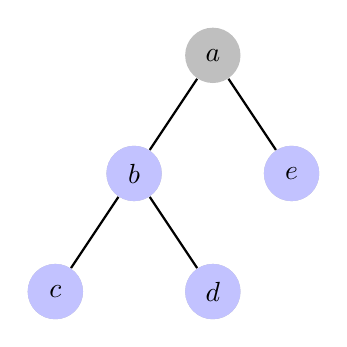
\begin{tikzpicture} [
                scale=1,
                vertex/.style={circle,fill=black!25,minimum size=20pt,inner sep=0pt},
                edge/.style = {draw,thick,-},
                selected vertex/.style = {vertex, fill=blue!24},
            ]
            \foreach \pos/\name in {
                    {(0,0)/c}, {(2,0)/d}, {(1,1.5)/b}, {(3,1.5)/e}, {(2,3)/a}}
                \node[vertex] (\name) at \pos {$\name$};
            \foreach \source/ \dest in {
                    b/c,b/d,a/b,a/e}
                \path[edge] (\source) edge (\dest);
            \foreach \vertex in {b,c,d,e}
                \path node[selected vertex] at (\vertex) {$\vertex$};
        \end{tikzpicture}
    \end{subfigure}
    \quad
    %%%%%%%%%%%%%%%%%%%%%%%%%%%%%%%%%%%%%%%%%%%%%%%%%%%%%%%%%%%%%%%%%%%%%%%%%%%%%%%%%%%%%
    \begin{subfigure}[b]{0.45\textwidth}
        \centering
        \caption{Sottografo (completo) indotto dai nodi dispari, e matching perfetto di costo minimo evidenziato}
        \label{fig:mchristmatching}
        \begin{tikzpicture} [
                scale=1,
                vertex/.style={circle,fill=black!25,minimum size=20pt,inner sep=0pt},
                edge/.style = {draw,thick,-},
                selected edge/.style = {draw,line width=5pt,-,blue!24},
            ]
            \foreach \pos/\name in {
                    {(0,0)/c}, {(2,0)/d}, {(1,1.5)/b}, {(3,1.5)/e}}
                \node[vertex] (\name) at \pos {$\name$};
            \foreach \source/ \dest in {
                    b/c,b/d,b/e,c/e,c/d,e/d}
                \path[edge] (\source) edge (\dest);
            \begin{pgfonlayer}{background}
                \foreach \source / \dest in {b/c,d/e}
                    \path[selected edge] (\source.center) -- (\dest.center);
            \end{pgfonlayer}
        \end{tikzpicture}
    \end{subfigure}
\end{figure}
    % \\[2pt]
% magic to split a figure https://tex.stackexchange.com/a/278748
\begin{figure}[htb]\ContinuedFloat
    \caption{Algoritmo di Christofides splittato in due pagine (cont.)}
    %%%%%%%%%%%%%%%%%%%%%%%%%%%%%%%%%%%%%%%%%%%%%%%%%%%%%%%%%%%%%%%%%%%%%%%%%%%%%%%%%%%%%
    \begin{subfigure}[b]{0.45\textwidth}
        \centering
        \caption{Ciclo Euleriano
            $ \langle c,b,d,e,a,b,c \rangle$
        }
        \label{fig:mchristeulertour}
        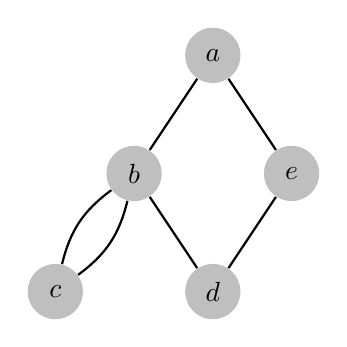
\begin{tikzpicture} [
                scale=1,
                vertex/.style={circle,fill=black!25,minimum size=20pt,inner sep=0pt},
                edge/.style = {draw,thick,-},
                bent right/.style = {bend right=20},
            ]
            \foreach \pos/\name in {
                    {(0,0)/c}, {(2,0)/d}, {(1,1.5)/b}, {(3,1.5)/e}, {(2,3)/a}}
                \node[vertex] (\name) at \pos {$\name$};
            \foreach \source/ \dest in {
                    b/d,a/b,a/e,d/e}
                \path[edge] (\source) edge (\dest);
            \foreach \source/ \dest in {
                    c/b,b/c}
                \path[edge] (\source) edge [bent right] (\dest);
        \end{tikzpicture}
    \end{subfigure}
    \quad
    %%%%%%%%%%%%%%%%%%%%%%%%%%%%%%%%%%%%%%%%%%%%%%%%%%%%%%%%%%%%%%%%%%%%%%%%%%%%%%%%%%%%%
    \begin{subfigure}[b]{0.45\textwidth}
        \centering
        \caption{Dopo lo \emph{shortcutting}:
            $ \langle c,b,d,e,a,\cancel{b},c \rangle$
        }
        \label{fig:mchristresult}
        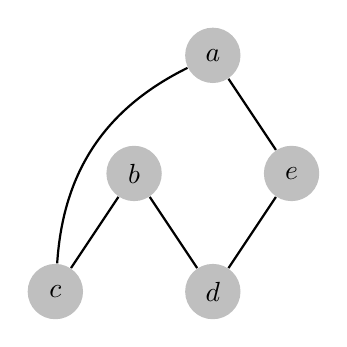
\begin{tikzpicture} [
                scale=1,
                vertex/.style={circle,fill=black!25,minimum size=20pt,inner sep=0pt},
                edge/.style = {draw,thick,-},
                bent right/.style = {bend right=30},
            ]
            \foreach \pos/\name in {
                    {(0,0)/c}, {(2,0)/d}, {(1,1.5)/b}, {(3,1.5)/e}, {(2,3)/a}}
                \node[vertex] (\name) at \pos {$\name$};
            \foreach \source/ \dest in {
                    b/d,a/e,d/e,b/c}
                \path[edge] (\source) edge (\dest);
            \foreach \source/ \dest in {
                    a/c}
                \path[edge] (\source) edge [bent right] (\dest);
        \end{tikzpicture}
    \end{subfigure}
\end{figure}

\lipsum{10}

\begin{figure}[h]
    \centering
    \caption{$3-CNF-SAT$ to $CLIQUE$}
    \label{fig:3cnfsatex}
    \begin{tikzpicture} [
            scale=1,
            vertex/.style={circle,fill=black!25,minimum size=20pt,inner sep=0pt},
            edge/.style = {draw,thin,-},
            outbound edge/.style = {draw,line width=4pt,-,blue!30},
            selected edge/.style = {draw,line width=4pt,-,red!30},
        ]
        % First we draw the vertices
        \foreach \pos/\name/\label in {
                % top left
                {(-1.5,5)/c/x_3},
                {(-2.5,3.5)/b/x_2},
                {(-3.5,2)/a/\bar{x_1}},
                % top right
                {(1.5,5)/d/x_1},
                {(2.5,3.5)/e/x_2},
                {(3.5,2)/f/\bar{x_3}},
                % bottom row
                {(2,0)/g/\bar{x_3}},
                {(0,0)/h/\bar{x_2}},
                {(-2,0)/i/x_1}}
            \node[vertex] (\name) at \pos {\name $\label$};
        % Connect vertices with edges
        \foreach \source/ \dest in {
                f/g,f/i,
                e/g,e/i,
                d/g,d/h,d/i,
                c/d,c/e,c/h,c/i,
                b/d,b/e,b/f,b/g,b/i,
                a/e,a/f,a/g,a/h}
            \path[edge] (\source) -- (\dest);
        % color some edges on background layer
        \begin{pgfonlayer}{background}
            \foreach \source / \dest in {c/d,d/i,i/c}
                \path[outbound edge] (\source.center) -- (\dest.center);
            \foreach \source / \dest in {a/e,e/g,g/a}
                \path[selected edge] (\source.center) -- (\dest.center);
        \end{pgfonlayer}
    \end{tikzpicture}
\end{figure}
